%%%%%%%%%%%%%%%%%%%%%%%%%%%%%%%%%%%%%%%%%
% a0poster Landscape Poster
% LaTeX Template
% Version 1.0 (22/06/13)
%
% The a0poster class was created by:
% Gerlinde Kettl and Matthias Weiser (tex@kettl.de)
% 
% This template has been downloaded from:
% http://www.LaTeXTemplates.com
%
% License:
% CC BY-NC-SA 3.0 (http://creativecommons.org/licenses/by-nc-sa/3.0/)
%
%%%%%%%%%%%%%%%%%%%%%%%%%%%%%%%%%%%%%%%%%

%----------------------------------------------------------------------------------------
%	PACKAGES AND OTHER DOCUMENT CONFIGURATIONS
%----------------------------------------------------------------------------------------

\documentclass[landscape]{a0poster}
\usepackage[fei]{common/theme} 	% základní styly
\usepackage{common/packages} 	% základní styly

\usepackage[sfdefault]{roboto}  %% Option 'sfdefault' only if the base font of the document is to be sans serif
%\usepackage[T1]{fontenc}
%\usepackage{listings}

%\usepackage[utf8]{inputenc}
%\usepackage{multicol} % This is so we can have multiple columns of text side-by-side
\columnsep=100pt % This is the amount of white space between the columns in the poster
\columnseprule=3pt % This is the thickness of the black line between the columns in the poster

%\usepackage[svgnames]{xcolor} % Specify colors by their 'svgnames', for a full list of all colors available see here: http://www.latextemplates.com/svgnames-colors

%\usepackage{times} % Use the times font
%\usepackage{palatino} % Uncomment to use the Palatino font

%\usepackage{graphicx} % Required for including images
\graphicspath{{images/}} % Location of the graphics files
\usepackage{booktabs} % Top and bottom rules for table
\usepackage[font=small,labelfont=bf]{caption} % Required for specifying captions to tables and figures
%\usepackage{amsfonts, amsmath, amsthm, amssymb} % For math fonts, symbols and environments
%\usepackage{wrapfig} % Allows wrapping text around tables and figures
%\usepackage{svg}


\topmargin -1in

\definecolor{lightgray}{HTML}{F2F2F2}

%\setlength{\columnseprule}{5pt}
\setlength{\columnseprule}{0pt}


\begin{document}

%----------------------------------------------------------------------------------------
%	POSTER HEADER 
%----------------------------------------------------------------------------------------

% The header is divided into three boxes:
% The first is 55% wide and houses the title, subtitle, names and university/organization
% The second is 25% wide and houses contact information
% The third is 19% wide and houses a logo for your university/organization or a photo of you
% The widths of these boxes can be easily edited to accommodate your content as you see fit


\hspace{-7ex}
\noindent\colorbox{lightgray} {
\hspace{+5ex}
\begin{minipage}[b]{0.75\linewidth}
\vspace{+7ex}
\veryHuge \color{MainColor} \textbf{FACULTY OF ELECTRICAL ENGINEERING
AND INFORMATICS} \color{Black}\\ % Title
\color{gray} \Huge{UNIVERSITY OF PARDUBICE}\\ % Subtitle
\huge \textit{Czech Republic}\\ % Author(s)

\end{minipage}
%
\begin{minipage}[b]{0.35\linewidth}
\vspace{+5ex}
\unilogoPoster
\vspace{+0ex}
\end{minipage}
}\\[1cm]


%%%%%%%%%%%%%%%%%%%%%


\begin{minipage}[b]{\linewidth}
\begin{center}
\veryHuge \color{MainColor} \textbf{Webalyt: Implemetation of Architecture for Capturing Web User Behaviours\\ With Feedback Propagation} \color{Black}
\\[1cm]
\color{gray}
\huge \textbf{Petr Filip \& Lukáš Čegan}\\ % Author(s)
\end{center}
\end{minipage}

%

\vspace{1cm} % A bit of extra whitespace between the header and poster content

%----------------------------------------------------------------------------------------

\begin{multicols}{3} % This is how many columns your poster will be broken into, a poster with many figures may benefit from less columns whereas a text-heavy poster benefits from more

%----------------------------------------------------------------------------------------
%	ABSTRACT
%----------------------------------------------------------------------------------------

\color{MainColor} 
\section*{ABSTRACT}
\color{black}

In the world of the Internet where people are consuming web-content,  more and more emphasis is placed on user friendliness of web-pages. It means increasing web-page usability and better user-experience. Increasing quality of user-experience (UX) is the task of UX developers. They should always base their work on the best practices and research. Each web-page has its own specificity and it leads to new challenges for the UX developers. One of the biggest issues is the problematic view of a web-page on specific devices with specific web-browser versions. Tools for capturing user behaviour are available, but there are issues with data ownership and with the development of new functionality. Actually, there are no free easily scalable and extendable products for user data gathering on the market.  
  In this paper, implementation of architecture (based on Spring Boot microservices) for capturing web user behaviours with feedback propagation is introduced. Architecture implementation is easily scalable and extendable. Webalyt is helpful for understanding user behaviour and improving user-experience. 



\color{MainColor} 
\section*{BACKGROUND}
\color{black}
One year ago, we proposed architecture called Webalyt, which is designed for web analysis. The architecture reflects needs such as data gathering, data extraction, transformation, processing and analysis. Gathered data are used for increasing user-experience, because  Hint module is designed for sending of a recommendations to a user's web browser. For example, according to the recommendation web browser can increase a font size.
\begin{center}\vspace{1cm}
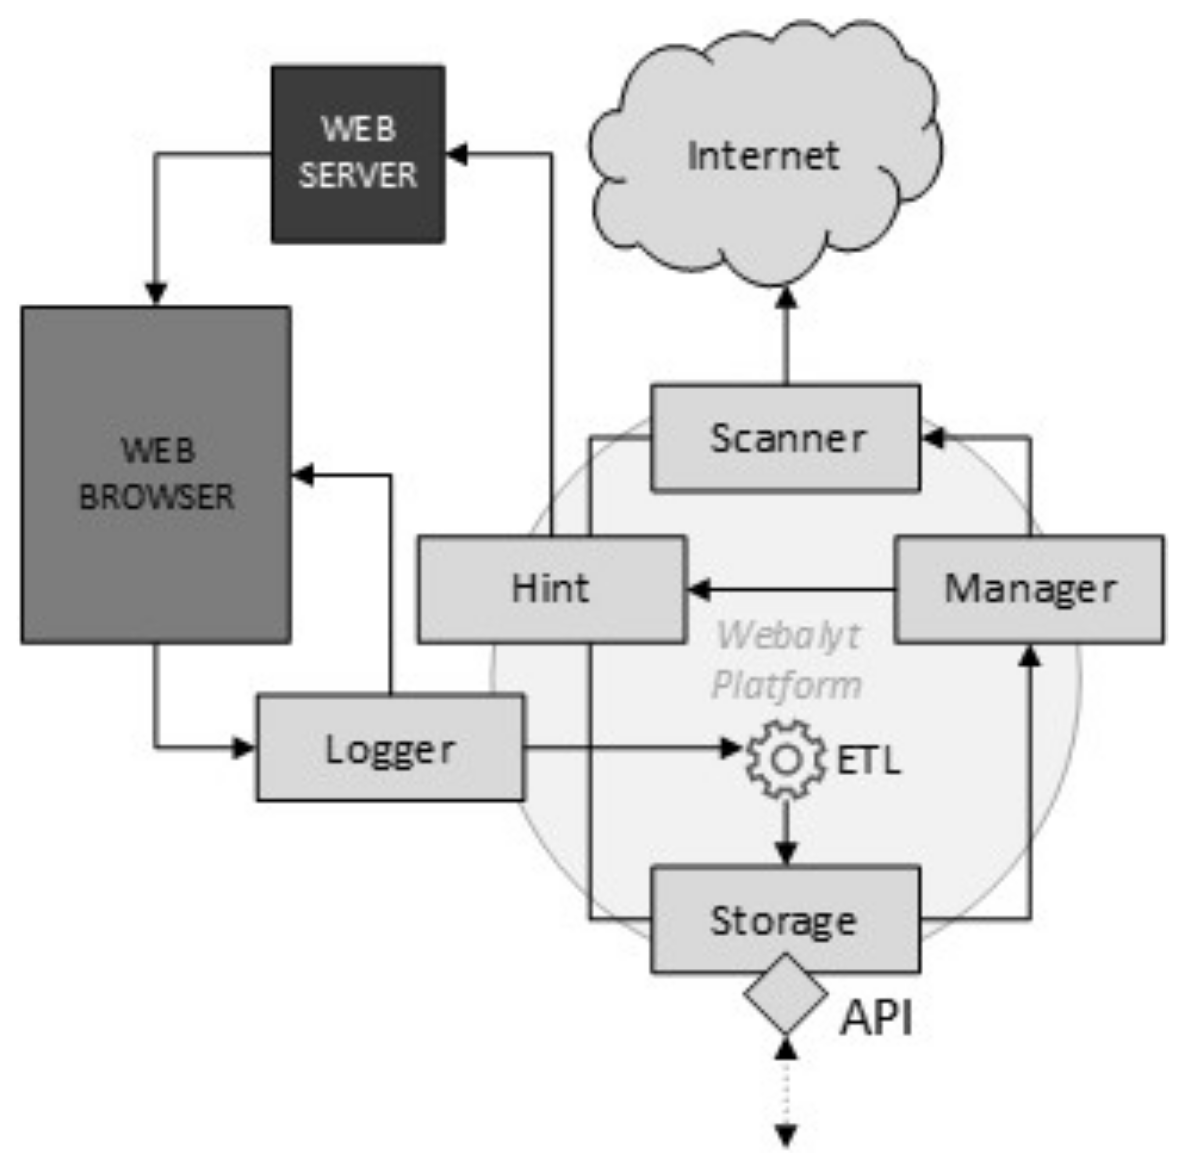
\includegraphics[width=0.60\columnwidth]{webalyt-architecture.png}
\color{MainColor}\captionof{figure}{\color{black} Proposed Webalyt Architecture}
\end{center}\vspace{1cm}


\vfill\null
\columnbreak 
 

\color{MainColor} 
\section*{IMPLEMENTATION}
\color{black}

Implemented system is Java based and lays on Spring Boot framework, Apache Kafka and Apache ZooKeeper. Many Spring Boot modules such as Spring Cloud Config, Eureka, Actuator, Kafka Streams were used. Due to used technologies and design patterns, architecture is easy scalable and maintainable.
% subsubsection  (end)



\begin{center}
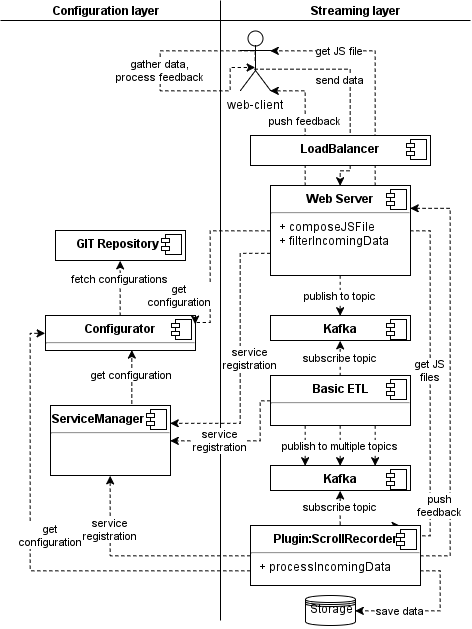
\includegraphics[width=0.90\columnwidth]{diagram-architecture-interaction}
\color{MainColor}\captionof{figure}{\color{black} Implementation of the Webalyt Architecture}
\end{center}\vspace{1cm}

%\vfill\null
%\columnbreak 
 
\color{MainColor} 
\subsection*{Data Layer}
\color{black}

\begin{center}
%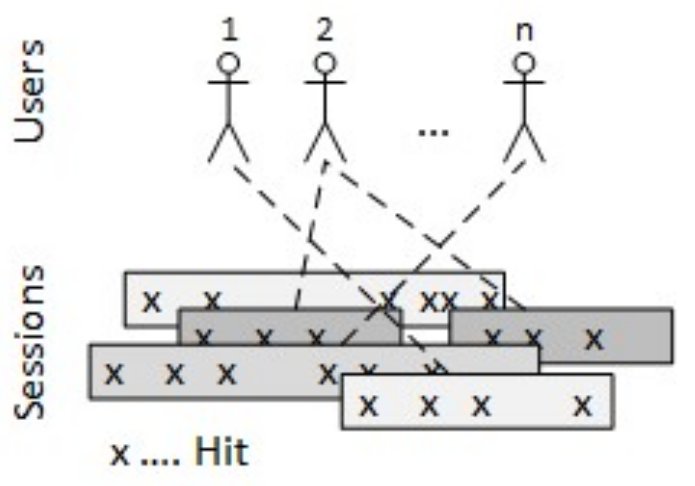
\includegraphics[width=0.4\columnwidth]{sessions-relations}  
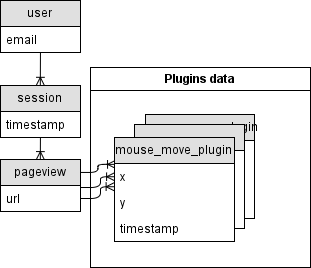
\includegraphics[width=0.4\columnwidth]{base-data-structure}
\color{MainColor}\captionof{figure}{\color{black} Data Structure}
\end{center}\vspace{1cm}


\color{MainColor} 
\subsection*{Plugin Skeleton}
\color{black}


\begin{center}
\begin{lstlisting}[label={lst_plugin_etl_code}]
@Service
public class MousePluginEtlService extends PluginBase<MousePosition> {
    @Override
    protected void processMessage(MousePosition object) {
		//implement the process logic
    }
}
\end{lstlisting}
\color{MainColor}\captionof{lstlisting}{\color{black} Plugin Skeleton Based on Spring Boot}
\end{center}\vspace{1cm}

\color{MainColor} 
\subsection*{ADVANTAGES}
\color{black}
\begin{itemize}
	\item easy to deploy and scale -- just run a JAR file
	\item easy to extend -- prepared skeleton for new modules
	\item self-hosted, optional cloud (AWS, Google Cloud)
	\item platform independent (Linux, Mac, Windows)
	\item open-source -- available on github
\end{itemize}


\color{MainColor} 
\section*{FORTHCOMING RESEARCH}
\color{black}
\begin{itemize}
	\item implementation of analytical and recommendation modules
	\item replaying of user session -- event such as scrolling, mouse movement, click etc.
	\item real-time remote control of a user session -- useful for a help-desk
	\item clustering of user -- based on user behaviour
\end{itemize}

%----------------------------------------------------------------------------------------
%	REFERENCES
%----------------------------------------------------------------------------------------

%\nocite{*} % Print all references regardless of whether they were cited in the poster or not
%\bibliographystyle{plain} % Plain referencing style
%\bibliography{sample} % Use the example bibliography file sample.bib


\end{multicols}




\vspace{+3ex}
\hspace{-7ex}
\noindent\colorbox{lightgray} {
\hspace{+5ex}
\begin{minipage}[b]{1.1\linewidth}
\vspace{+4ex}

\color{gray} \huge{
28th International Conference Radioelektronika 2018 - April 19 -20, 2018, Prague, Czech Republic
}\\ % Subtitle


\end{minipage}
}


\end{document}